\documentclass[tikz]{standalone}

\begin{document}
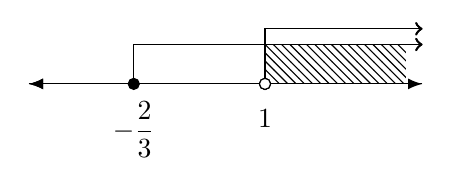
\begin{tikzpicture}[scale=1.0]

\usetikzlibrary{patterns}
\draw[-latex] (-2, 0) -- (3, 0);
\draw[latex-] (-2, 0) -- (3, 0);
\filldraw (-2/3, 0) circle (2pt);
\node [below] at (-2/3,-0.1) {$-\displaystyle\frac{2}{3}$};
\draw[->] (-2/3, 0) -- (-2/3, 0.5) -- (3, 0.5);
\filldraw[fill=white] (1, 0) circle (2pt);
\node [below] at (1,-0.2) {$1$};
\draw[->] (1, 0) -- (1, 0.7) -- (3, 0.7);
\filldraw[fill=white] (1, 0) circle (2pt);
\draw[white,pattern=north west lines] (1, 0) -- (1, 0.5) -- (2.8, 0.5) -- (2.8, 0) -- (-2/3, 0);
\draw[latex-] (-2, 0) -- (3, 0);
\draw[->] (1, 0) -- (1, 0.7) -- (3, 0.7);
\draw[->] (-2/3, 0) -- (-2/3, 0.5) -- (3, 0.5);
\filldraw[fill=white] (1, 0) circle (2pt);

\end{tikzpicture}
\end{document}